\subsection{Diseño/sintesis}

Con los analisis anteriores se buscaron los valores de componentes mediante la tecnica de igualacion de coeficientes y siguiendo las recomendaciones de el Daryanani.

\subsubsection{Realimentacion positiva (Sallen-Key)}

\noindent $>>$ \texttt{Recordando la FT \ref{posFT} e igualando a la funcion de transferencia requerida para la primer etapa, se obtienen las ecuaciones de diseño:}

\begin{align*}
    G &= \frac{k_1 s}{s^{2} + a_1 s + b_1} = \frac{5252.26 s}{s^{2} + 3184.42 s + 66320656} \\\\
    k_1 &= \frac{k}{C_{1} R_{1}} \\
    a_1 &= \frac{1}{C_{2} R_{3}} + \frac{1}{C_{1} R_{3}} - \frac{k}{C_{1} R_{2}} + \frac{1}{C_{1} R_{2}} + \frac{1}{C_{1} R_{1}} \\
    b_1 &= \frac{1}{C_{1} C_{2} R_{2} R_{3}} + \frac{1}{C_{1} C_{2} R_{1} R_{3}}
\end{align*}

\noindent $>>$ \texttt{En las que se tiene mas incognitas que ecuaciones, por lo que se siguieron las condiciones propuestas por el Daryanani:}

\begin{figure}[H]
    \centering
    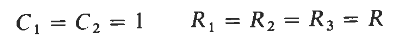
\includegraphics[scale=.8]{Secciones/Circ1/img/daryanani286.png}
    \caption{Seleccion de grados de libertad (Daryanani pag. 286).}
    \label{pv1}
\end{figure}

\noindent $>>$ \texttt{Sin considerar la ganancia k0 (que se ajusto mas tarde), aplicando las condiciones se obtuvieron las ecuaciones de sintesis:}

\begin{align*}
    - \frac{k}{R} + \frac{4}{R} &= 3184.42 \\
    \frac{2}{R^{2}} &= 66320656
\end{align*}

\noindent $>>$ \texttt{Resolviendo el sistema y escalando R para que C sea de 100nF:}

\begin{align*}
    C_{1} &= 100 nF \\
    C_{2} &= 100 nF \\
    R &= 1736.56 \\
    k &= 3.45 = 1+\frac{r_2}{r_1}
\end{align*}

Para la implementacion se decidio hacer R$\cong 1738 \Omega$ (implementanda con una red serie $1.5k\Omega+220\Omega+18\Omega$).

Y k$\cong 3.44$, con $(r_{1}=1k\Omega$ y $r_2=2440\Omega$ (implementada con red mixta $2.2k\Omega+720//720//720\Omega$).

% -----------------------------------
\subsubsection{Realimentacion negativa}

\noindent $>>$ \texttt{Recordando la FT \ref{negFT} e igualando a la funcion de transferencia requerida para la segunda etapa, se obtienen las ecuaciones de diseño:}

\begin{align*}
    G &= \frac{k_2 s}{s^{2} + a_2 s + b_2} = \frac{-3126.49 s}{s^{2} + 1895.58 s + 23500096} \\\\
    k_2 &= -\frac{1}{C_{2} R_{1}} \\
    a_2 &= \frac{1}{C_{2} R_{2}} + \frac{1}{C_{1} R_{2}} \\
    b_2 &= \frac{1}{C_{1} C_{2} R_{1} R_{2}}
\end{align*}

Para este caso tenemos una ganancia negativa propia del amplificador inversor, para resolver esto el ajuste de ganancia se implemento con un aplificador inversor en la ultima etapa del filtro. \\

\noindent $>>$ \texttt{Nuevamente se tiene mas incognitas que ecuaciones, por lo que se siguieron las condiciones propuestas por el Daryanani:}

\begin{figure}[H]
    \centering
    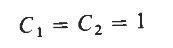
\includegraphics[scale=.8]{Secciones/Circ1/img/daryanani302.png}
    \caption{Seleccion de grados de libertad (Daryanani pag. 302).}
    \label{pv1}
\end{figure}

\noindent $>>$ \texttt{Sin considerar la ganancia k1, aplicando las condiciones se obtuvieron las ecuaciones de sintesis:}

\begin{align*}
    \frac{2}{R_{2}} &= 1895.58 \\
    \frac{1}{R_{1} R_{2}} &= 23500096
\end{align*}

\noindent $>>$ \texttt{Se resolvio el sistema y se escalaron resistencias para que C sea de 100nF:}

\begin{align*}
    C_{1} &= 100 nF \\
    C_{2} &= 100 nF \\
    R_1 &= 403.31 \\
    R_2 &= 10550.86 \Omega
\end{align*}

Para la implementacion se decidio hacer $R_1\cong 410\Omega$ (implementanda con una red paralelo $820//820\Omega$).

Y $R_2\cong 10560\Omega$ (implementada con red serie $10k\Omega+560\Omega$).